\documentclass{ComputationalAlgorithmsArticle}

\usepackage[dvips]{graphicx}
\usepackage{float}
\usepackage{subfigure}

\usepackage[dvips,
bookmarks,
bookmarksopen,
backref,
colorlinks,linkcolor={blue},citecolor={blue},urlcolor={blue},
]{hyperref}

\title{Visualizing Differences Between Two VTK Meshes}

% 
% NOTE: This is the last number of the "handle" URL that 
% The Insight Journal assigns to your paper as part of the
% submission process. Please replace the number "1338" with
% the actual handle number that you get assigned.
%
\newcommand{\IJhandlerIDnumber}{3303}

% Increment the release number whenever significant changes are made.
% The author and/or editor can define 'significant' however they like.
\release{0.00}

% At minimum, give your name and an email address.  You can include a
% snail-mail address if you like.

\author{David Doria and Adam Gerlach}
\authoraddress{Rensselaer Polytechnic Institute}


\begin{document}

\IJhandlefooter{\IJhandlerIDnumber}


\ifpdf
\else
   %
   % Commands for including Graphics when using latex
   % 
   \DeclareGraphicsExtensions{.eps,.jpg,.gif,.tiff,.bmp,.png}
   \DeclareGraphicsRule{.jpg}{eps}{.jpg.bb}{`convert #1 eps:-}
   \DeclareGraphicsRule{.gif}{eps}{.gif.bb}{`convert #1 eps:-}
   \DeclareGraphicsRule{.tiff}{eps}{.tiff.bb}{`convert #1 eps:-}
   \DeclareGraphicsRule{.bmp}{eps}{.bmp.bb}{`convert #1 eps:-}
   \DeclareGraphicsRule{.png}{eps}{.png.bb}{`convert #1 eps:-}
\fi


\maketitle


\ifhtml
\chapter*{Front Matter\label{front}}
\fi

\begin{abstract}
\noindent

This document presents two methods of computing and visualizing the differences between to vtkPolyData mesh objects. One method, vtkPolyDataDelta, relies on reasonable normal estimates, while the other, vtkMeshPointDifference, does not.

The code is available here:
\begin{verbatim}
https://github.com/agerlach/vtkPolyDataDelta
\end{verbatim}


\end{abstract}

\IJhandlenote{\IJhandlerIDnumber}

\tableofcontents
%%%%%%%%%%%%%%%%%%%%
\section{Introduction}
When two meshes represent the same physical object, it is informative to be able to compare them in a qualitative way.
We do this by visualizing the difference between them by coloring the surface based on the "difference" between
the meshes. We present two methods of computing and visualizing the differences between to vtkPolyData mesh objects. One method (vtkPolyDataDelta) relies on reasonable normal estimates, while the other does not. When the normals are known, the distance is computed by "shooting" the normal of every point of mesh A and finding its intersection with mesh B. When the normals are not known (vtkMeshPointDifference), the closest point on mesh A is found from every point on mesh B. In both cases, these distances are mapped to colors and these colors are applied to the mesh for visualization of the computations.

\section{Included Files}
\begin{itemize}
\item vtkPolyDataDeltaDemo programmatically creates two meshes with known normals and compares them.
\item vtkPolyDataDeltaExample reads two meshes with known normals from vtp files and compares them.
\item vtkMeshPointDifferenceDemo programmatically creates two meshes with unknown normals and compares them.
\item vtkMeshPointDifferenceExample reads two meshes with unknown normals from vtp files and compares them.
\end{itemize}


%%%%%%%%%%%%%%%%%%%%
\section{Difference Computation with Normals}
The distance to mesh A is found by shooting the normal from every point of mesh B and determining its intersection with mesh A. A Modified BSP tree is used to speed up this ray/triangle intersection computation.

Figure \ref{fig:RayIntersection} explains this distance computation graphically.

\begin{figure}[H]
  \centering
  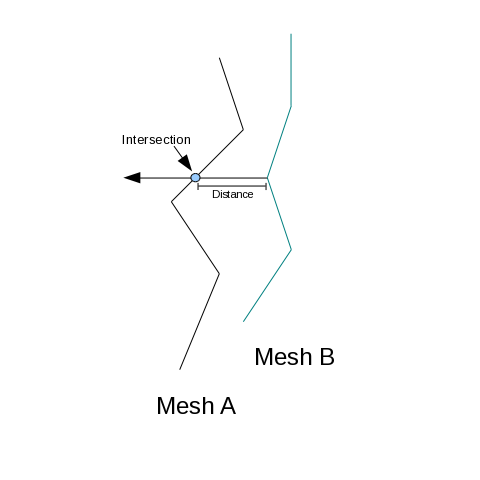
\includegraphics[width=0.5\linewidth]{images/RayIntersection}
  \caption{A graphical explanation of the normal intersection distance computation.}
  \label{fig:RayIntersection}
\end{figure}

%%%%%%%%%%%%%%%%%%%%
\section{Difference Computation without Normals}
The closest point in mesh A is found from every point of mesh B. The distance between these points is taken as the distance between the two meshes at that point. A KD-Tree is used to speed up this nearest neighbor lookup.

Figure \ref{fig:NearestNeighbor} explains this distance computation graphically.

\begin{figure}[H]
  \centering
  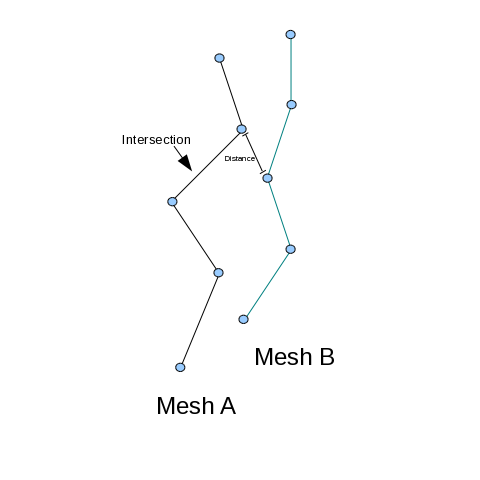
\includegraphics[width=0.5\linewidth]{images/NearestNeighbor}
  \caption{A graphical explanation of the nearest neighbor distance computation.}
  \label{fig:NearestNeighbor}
\end{figure}

\end{document}
